\documentclass{beamer}

\mode<presentation> {
\usetheme{AnnArbor}
}

\usepackage{graphicx}
\graphicspath{{./figures/}}
\usepackage{caption}
\usepackage{subcaption}
\usepackage{hyperref}
\hypersetup{colorlinks=true}
\usepackage{amsmath}
\usepackage{amsthm}
\usepackage{multirow}
\usepackage{siunitx}
\usepackage{biblatex}
\addbibresource{bibliography.bib}

\AtEveryBibitem{
    \clearfield{doi}
    \clearfield{isbn}
    \clearfield{issn}
    \clearlist{language}
    \clearfield{note}
    \clearfield{url}
    \clearfield{urlyear}
}

\setbeamertemplate{caption}[numbered]

\newtheorem{assumption}{Assumption}[section]
\newtheorem{proposition}{Proposition}
\newtheorem{remark}{Remark}[section]
\def\C{\mathbb C}
\def\P{\mathbb P}
\def\R{\mathbb R}
\def\Z{{\mathbb Z}}
\def\sign{{\rm sign}}
\def\ind{\perp\!\!\!\perp}
\DeclareMathOperator*{\argmin}{arg\,min}
\DeclareMathOperator*{\argmax}{arg\,max}

\title[Forecasting the Solar X-Ray Flux]{Forecasting the Solar X-Ray Flux}

\author{Victor Verma, Yang Chen, Stilian Stoev}
\institute[]
{
Department of Statistics \\
University of Michigan
}
\date[6/22/23]{6/22/23}

\begin{document}

\begin{frame}
    \titlepage
\end{frame}

\begin{frame}{Outline}
   \tableofcontents
\end{frame}

\section{Introduction}

\begin{frame}{Background on Solar Flares}
    \begin{itemize}
        \item A solar flare is a sudden, massive eruption of electromagnetic radiation from the Sun's atmosphere.
        \item Adverse effects of solar flares: 
        \begin{itemize}
            \item Radio blackouts
            \item Coronal mass ejection (CME) $\rightarrow$ electromagnetic pulse $\rightarrow$ electrical blackouts
            \item Solar energetic particle event (SEP) $\rightarrow$ irradiation of astronauts
        \end{itemize}
        \item Some notable incidents:
        \begin{itemize}
            \item 1859: The Carrington flare, one of the most extreme ever recorded
            \item 1989: The electrical grid in Quebec was shut down for several hours
            \item 2022: Dozens of Starlink satellites were destroyed
        \end{itemize}
    \end{itemize}
\end{frame}

\begin{frame}{Flare Strength}
    Flare strength is determined by the peak soft X-ray flux.
    \begin{table}
        \centering
        \begin{tabular}{|c|c|}
            \hline
            Flare Class & X-Ray Flux Threshold ($\text{W} / \text{m}^2$) \\
            \hline
            A & $10^{-8}$ \\
            B & $10^{-7}$ \\
            C & $10^{-6}$ \\
            M & $10^{-5}$ \\
            X & $10^{-4}$ \\
            \hline
        \end{tabular}
        \caption{X-ray flux thresholds for the different flare classes}
        \label{tab:flare_classes}
    \end{table}

    Goal:
    \begin{center}
        Forecast flares by predicting whether the flux will be above a threshold
    \end{center}
\end{frame}

\begin{frame}{Existing Work}
    Example: Deep Flare Net \cite{nishizuka2018deep, nishizuka2021oper}
    \begin{itemize}
        % \item A feedforward neural network
        \item Predicts whether strong flare will occur in next 24 hours
        % Unclear whether GOES data is science-quality
        % \item Uses features based on the X-ray flux and images (magnetograms, EUV images) of the Sun
        % \item Was trained on 2010-2014 data, was tested on 2015 data
        % \item Entered service in Japan's space weather forecasting office in 2019, was tested on data from 1/19-6/20
        \item For M+ class flares, non-operational TSS = 0.8, operational = 0.24
    \end{itemize}    
    The flare forecasting problem has not been solved:
    \begin{itemize}
        % \item High TSS values have been achieved in non-operational settings, but not in operational settings
        \item Forecasting methods were compared in operational setting in \cite{leka2019acomII, leka2019acomIII}
        \item Goal: predict if C+ class or M+ class flare will occur in next 24 hours
        \item For both, no method attained a TSS over 0.5.
        % \item The U.S. Space Weather Prediction Center's approach had a TSS of 0.3 for M class flares
        \item ML-based methods tended to perform worse
    \end{itemize}
\end{frame}

\section{Foundations of Optimal Extreme Event Prediction}

\begin{frame}{A General Characterization of Optimal Predictors}
    Let $Y$ be a random variable with a continuous CDF $F_Y$ and $X$ a random vector in $\R^d$. We make the following technical assumption:
    \begin{assumption}\label{assump:joint_dens}
        $X$ and $Y$ have a joint density $f$ with respect to the Lebesgue measure on $\R^d \times \mathbb{R}$.
    \end{assumption}
    The flare forecasting problem is an instance of this general problem:
    \begin{center}
        Predict whether $Y > F_Y^{-1}(p_0)$ using $h(X)$ for some suitable $h$.
    \end{center}
\end{frame}

\begin{frame}{A General Characterization of Optimal Predictors}
    % Say "predict", or "raise an alarm"
    Given $h$, we predict that $Y > F_Y^{-1}(p_0)$ when $h(X)$ lies in some set $S$.

    Indicators can be used to represent the predictand and a predictor:
    \[
    I(Y > F_Y^{-1}(p_0)), I(h(X) \in S)
    \]

    % Obvious choice for $q_0$: $p_0$, explain why. Obvious choice for $S$ when p_0 = q_0: $(F_{h(X)}^{-1}(p_0), \infty)$. Explain why we might not want q_0 = p_0.
    Predictors should be calibrated:
    \begin{definition}
        $I(h(X) \in S)$ is a predictor of $I(Y > F_Y^{-1}(p_0))$ that is calibrated at level $q_0$ if 
        \[
        P(h(X) \in S) = 1 - q_0.
        \]
    \end{definition}
\end{frame}

\begin{frame}{A General Characterization of Optimal Predictors}
    Certain predictors can be viewed as optimal: 
    \begin{definition}\label{d:opt-pred}
        $I(h(X) \in S)$ is an optimal predictor of $I(Y > F_Y^{-1}(p_0))$ at level $q_0$ if
        \begin{itemize}
            \item it is calibrated at level $q_0$
            \item for any other predictor $I(k(X) \in T)$ that is calibrated at level $q_0$,
            \begin{equation}\label{eq:optimality_cond}
            P(Y > F_Y^{-1}(p_0) \mid h(X) \in S) \ge P(Y > F_Y^{-1}(p_0) \mid k(X) \in T)
            \end{equation}
        \end{itemize}
        The two probabilities in \eqref{eq:optimality_cond} are denoted $\lambda_{p_0, q_0}(Y, h(X))$ and $\lambda_{p_0, q_0}(Y, k(X))$, respectively.
    \end{definition}
\end{frame}

\begin{frame}{A General Characterization of Optimal Predictors}
    Let
    \begin{itemize}
        \item $f_0$ be the conditional density of $X$ given that $Y \le F_Y^{-1}(p_0)$
        \item $f_1$ the conditional density of $X$ given that $Y > F_Y^{-1}(p_0)$
    \end{itemize}
    Then
    \begin{align*}
        f_0(x) &= \frac{1}{p_0}\int_{-\infty}^{F_Y^{-1}(p_0)} f(x, y)\,dy \\
        f_1(x) &= \frac{1}{1 - p_0}\int_{F_Y^{-1}(p_0)}^{\infty} f(x, y)\,dy
    \end{align*}

    % Say that it is potentially difficult to estimate r(x)
    \begin{theorem}\label{thm:base_thm}
        Let $r(x) = f_1(x) / f_0(x)$. Then $I(r(X) > F_{r(X)}^{-1}(q_0))$ is an optimal predictor of $I(Y > F_Y^{-1}(p_0))$ at level $q_0$, i.e., Relation \eqref{eq:optimality_cond} holds.
    \end{theorem}
\end{frame}

\begin{frame}{Examples of Optimal Extreme Event Predictors}
    \begin{theorem}[Linear heteroskedastic models]\label{thm:add_err_mod_thm}
        Let $X \in \R^d$ and $\epsilon \in \R$ be independent and let $\sigma$ be a function that is positive on the range of $X$. Suppose that 
        \begin{equation}\label{e:thm:add_err_mod_thm}
        Y = g(X) + \sigma(X)\epsilon.
        \end{equation}
        Also suppose that Assumption~\ref{assump:joint_dens} holds. Let $p_0 \in (0, 1)$. Then an optimal predictor of $I(Y > F_Y^{-1}(p_0))$ at level $q_0$ is $I(k(X) \ge \tau_0)$, where
        \[
        k(X) = \frac{g(X) - F_Y^{-1}(p_0)}{\sigma(X)}
        \]
        and $\tau_0$ is some suitably chosen constant that calibrates the predictor.
    \end{theorem}
\end{frame}

\begin{frame}{Examples of Optimal Extreme Event Predictors}
    \begin{corollary}
        When $\sigma(X)$ in \eqref{e:thm:add_err_mod_thm} is constant with respect to $X$, then an optimal predictor is
        \[
        I(g(X) \ge \tau_0)
        \]
        for some constant $\tau_0$ that calibrates the predictor.
    \end{corollary}

    \begin{proposition} \label{p:monotone-link}
        Let $Y = g(X + \delta) + \epsilon$, where $X,\ \delta$ and $\epsilon$ are independent random
        variables. If $g$ is a non-decreasing function, then the optimal predictor of $I(Y > F^{-1}(p_0))$ is of the form $I(X > \tau_0)$, $\tau_0$ being a constant that calibrates the predictor.
    \end{proposition}
    % Say that these results can be used to derive optimal predictors for time series models.
\end{frame}

\begin{frame}{Performance Metrics}
    \begin{table}[h]
        \centering
        \begin{tabular}{@{}cc|cc@{}}
            \multicolumn{1}{c}{} &\multicolumn{1}{c}{} &\multicolumn{2}{c}{Observed} \\ 
            \multicolumn{1}{c}{} & 
            \multicolumn{1}{c|}{} & 
            \multicolumn{1}{c}{Yes} & 
            \multicolumn{1}{c}{No} \\ 
            \cline{2-4}
            \multirow[c]{2}{*}{Predicted} % Had \rotatebox[origin=tr]{90}{Predicted} instead of Predicted, but text overlapped
            & Yes  & TP & FP   \\[1.5ex]
            & No  & FN   & TN \\ 
            \cline{2-4}
        \end{tabular}
        \caption{A confusion matrix.}
        \label{tab:conf_mat}
    \end{table}
    Definitions of the precision, true positive rate (TPR), and false positive rate (FPR) of a predictor:
    \[
    \text{Precision} := \frac{TP}{TP + FP}, \
    TPR := \frac{TP}{TP + FN}, \
    FPR := \frac{FP}{FP + TN}
    \]
\end{frame}

\begin{frame}{Performance Metrics}
    Since
    \begin{align*}
        \lambda_{p_0, q_0}(Y, k(X)) &= P(Y > F_Y^{-1}(p_0) \mid k(X) \in T),
    \end{align*}
    we call $\lambda_{p_0, q_0}(Y, k(X))$ the precision of $I(k(X) \in T)$.

    \medskip
    
    If $I(h(X) \in S)$ is optimal, then we call $\lambda_{p_0, q_0}(Y, h(X))$ the optimal precision.

    \medskip
    
    If $p_0 = q_0$, then we call the limits
    \[
    \lim_{p_0 \uparrow 1} \lambda_{p_0, p_0}(Y, k(X)) \text{ and } \lim_{p_0 \uparrow 1} \lambda_{p_0, p_0}(Y, h(X))
    \]
    the asymptotic precision for $I(k(X) \in T)$ and the asymptotic optimal precision, respectively.
\end{frame}

\begin{frame}{Performance Metrics}
    We call
    \[
    P(k(X) \in T \mid Y > F_Y^{-1}(p_0)), P(k(X) \in T \mid Y \le F_Y^{-1}(p_0))
    \]
    the true positive rate (TPR) and false positive rate (FPR), respectively.

    \medskip
    
    We can express these in terms of $\lambda_{p_0, q_0}$, $p_0$, and $q_0$:
    \begin{align*}
        TPR &= \frac{\lambda_{p_0, q_0}(1 - q_0)}{1 - p_0} \\
        FPR &= \frac{(1 - \lambda_{p_0, q_0})(1 - q_0)}{p_0}
    \end{align*}
\end{frame}

\begin{frame}{Performance Metrics}
    Many metrics are used to evaluate predictor performance. Two examples are the TSS and the F1 score. Letting $\lambda = \lambda_{p_0, q_0}$, we have
    \[
    \text{TSS} = \text{TPR} - \text{FPR} = \frac{\lambda(1 - q_0)}{1 - p_0} - \frac{(1 - \lambda)(1 - q_0)}{p_0} = \frac{1 - q_0}{p_0(1 - p_0)}\lambda - \frac{1 - q_0}{p_0}
    \]
    and
    \[
    \text{F1} = \frac{2\lambda \cdot \text{TPR}}{\lambda + \text{TPR}} = \left.\frac{2\lambda^2(1 - q_0)}{1 - p_0} \middle/ \left[\lambda + \frac{\lambda(1 - q_0)}{1 - p_0}\right]\right. = \frac{2(1 - q_0)}{2 - p_0 - q_0}\lambda
    \]
    so maximizing the precision is equivalent to maximizing the TSS and the F1 score.
\end{frame}

\begin{frame}{Performance Metrics}
    Let $X$ and $Y$ be random variables. The level-$p_0$ tail dependence coefficient $\lambda_{p_0} = \lambda_{p_0}(Y, X)$ is defined by
    \begin{align*}
        \lambda_{p_0} &:= P(Y > F_Y^{-1}(p_0) \mid X > F_X^{-1}(p_0)) \\
        &:= \frac{P(Y > F_Y^{-1}(p_0)), X > F_X^{-1}(p_0)}{1 - p_0},
    \end{align*}
    and the tail dependence coefficient $\lambda = \lambda(X, Y)$ is defined by
    \[
    \lambda := \lim_{p_0 \uparrow 1} \lambda_{p_0}
    \]
    if the limit exists.
\end{frame}

\begin{frame}{ROC Dominance Property}
    \begin{definition}
        A family $\mathcal{F}(k)$ of predictors of $I(Y > F_Y^{-1}(p_0))$ is a set of the form
        \[
        \{I(k(X) > F_{k(X)}^{-1}(q_0) : 0 \le q_0 \le 1\}.
        \]
        We denote the precision, the TPR, and the FPR for a member of this family by $\lambda(q_0)$, $TPR(q_0)$, and $FPR(q_0)$, respectively.
    \end{definition}

    \begin{definition}
        The ROC curve of the family $\mathcal{F}(k)$ is defined as 
        \[
        R(k) := \{(FPR(q_0), TPR(q_0)) : 0 \le q_0 \le 1\}.
        \]
    \end{definition}    
\end{frame}

\begin{frame}{ROC Dominance Property}
    \begin{definition}    
        The suboptimality region of the family $\mathcal{F}(k)$ is defined as
        \[
        D(k) := \bigcup_{q_0 \in [0, 1]} \{(FPR, TPR(q_0)) : FPR \ge FPR(q_0)\}.
        \]
    \end{definition}
    
    \begin{definition}
        Given two families $\mathcal{F}(k)$ and $\mathcal{F}(\ell)$ of predictors of $I(Y > F_Y^{-1}(p_0))$, we say that $\mathcal{F}(k)$ dominates $\mathcal{F}(\ell)$ in ROC order if
        \[
        D(k) \supseteq D(\ell).
        \]
        In this case, we write
        \[
        \mathcal{F}(k) \ge_{ROC} \mathcal{F}(\ell).
        \]
    \end{definition}
\end{frame}

\begin{frame}{ROC Dominance Property}
    \begin{proposition}
        Let $\mathcal{F} = \mathcal{F}(k)$ and $\mathcal{F}^* = \mathcal{F}(h)$ be two families of predictors of $I(Y > F_Y^{-1}(p_0))$, with the latter consisting of optimal predictors.

        \medskip
        
        Let $TPR^*(q_0)$ represent the true positive rates for $\mathcal{F}^*$.

        \medskip

        If $TPR^*$ is strictly decreasing, then $\mathcal{F}^* \ge_{ROC} \mathcal{F}$.
    \end{proposition}
\end{frame}

\begin{frame}{ROC Dominance Property}
    \begin{figure}[h!]
        \centering
        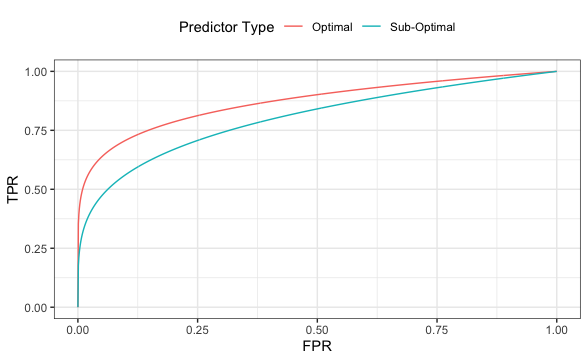
\includegraphics[scale=0.4]{roc_curves.png}
        \caption{ROC Curves.}
        \label{fig:roc_curves}
    \end{figure}
\end{frame}

\begin{frame}{Data Information}
    \begin{itemize}
        \item Response (X-ray flux) data comes from the GOES satellites.
        % \begin{itemize}
        %     \item We use science-quality data, not operational data.
        %     \item The data is on a one-minute cadence.
        %     \item The data is mostly from solar cycle 24 (2008-2019), which saw unusually low levels of solar activity \cite{noaa2020hell}.
        % \end{itemize}
        \item Covariate (SHARP parameter) data comes from the Solar Dynamics Observatory (SDO).
        % \begin{itemize}
        %     \item Raw covariates are SHARP parameters, variables that describe flare-producing active regions in various ways \cite{bobra2014theh}.
        %     \item The data is on a 12-minute cadence.
        % \end{itemize}
    \end{itemize}

    The response and covariate data was combined as follows:
    \begin{itemize}
        \item Impute missing flux and SHARP parameter values
        % by taking the maximum across active regions at each time
        \item Aggregate SHARP parameter data across HARPs 
        \item Join aggregated SHARP time series to flux time series
    \end{itemize}
    The final time series consists of $\num[group-separator={,}]{287635}$ observations.
\end{frame}

\begin{frame}{X-Ray Flux Data}
    \begin{figure}
        \centering
        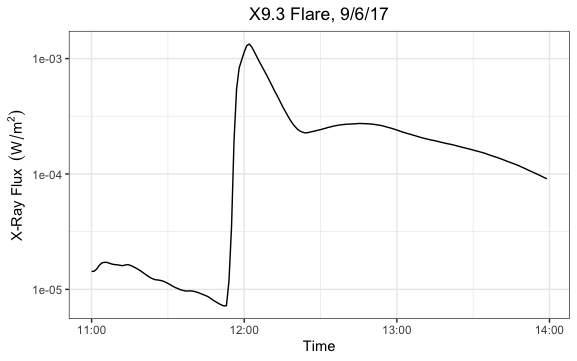
\includegraphics[scale=0.5]{flare_flux_example.png}
        \caption{The X-ray flux for an X-class flare}
        \label{fig:flare_flux_example}
    \end{figure}
\end{frame}

\begin{frame}{X-Ray Flux Data}
    \begin{itemize}
        \item The flux level is measured by the Geostationary Orbiting Environmental Satellites (GOES).
        \item We use data from the GOES-15 satellite, which has data from 3/31/10-3/4/20.
        \item The flux is measured every 2s; we use 1m averages.
    \end{itemize}
\end{frame}

\begin{frame}{X-Ray Flux Data}
    \begin{figure}
        \centering
        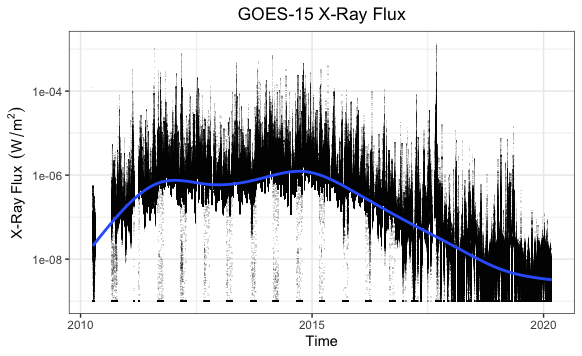
\includegraphics[scale=0.5]{flux_time_series.png}
        \caption{The GOES-15 X-Ray flux time series}
        \label{fig:flux_time_series}
    \end{figure}
\end{frame}

\begin{frame}{X-Ray Flux Data}
    \begin{figure}
        \centering
        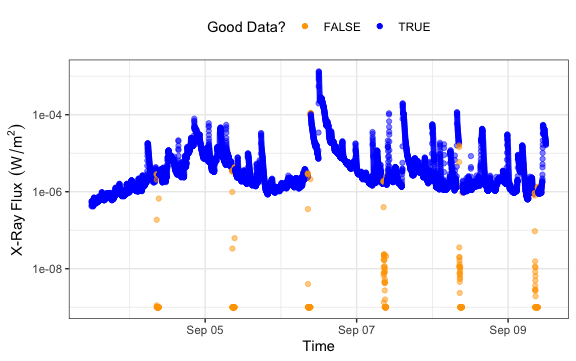
\includegraphics[scale=0.5]{flux_20170906.png}
        \caption{The X-Ray flux, 9/3/17-9/9/17.}
        \label{fig:flux_20170906}
    \end{figure}
\end{frame}

\begin{frame}{X-Ray Flux Data}
    \begin{figure}
        \centering
        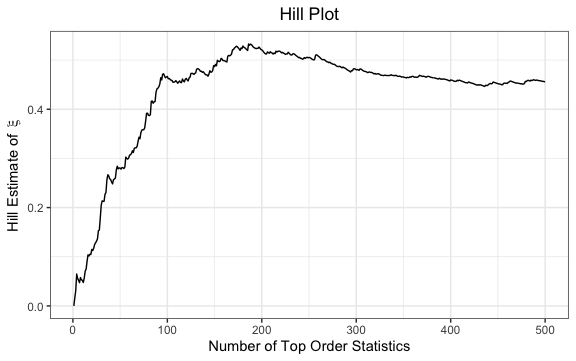
\includegraphics[scale=0.5]{hill_plot.png}
        \caption{A Hill plot for the X-Ray flux.}
        \label{fig:hill_plot}
    \end{figure}
\end{frame}

\begin{frame}{SHARP Parameter Data}
    Solar flares typically emerge from active regions, areas of the solar atmosphere  characterized by intense magnetic activity.
    \begin{figure}
        \centering
        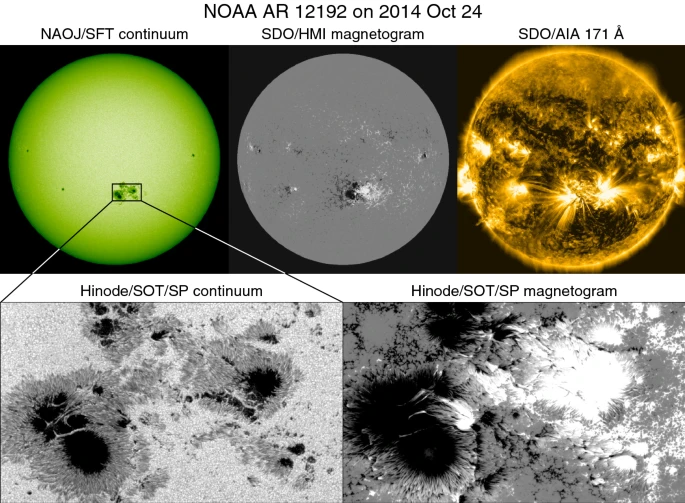
\includegraphics[scale=0.33]{active_region.png}
        \caption{Source: \cite{toriumi2019flar}}
        \label{fig:active_region}
    \end{figure}
\end{frame} 

\begin{frame}{SHARP Parameter Data}
    \begin{itemize}
        \item SHARP (Spaceweather HMI Active Region Patch) parameters are variables that describe active regions.
        \item An HMI Active Region Patch (HARP) is an automatically-delineated area that encloses an active region.
        \item We use SHARP data from 5/1/10-6/24/18.
        \item SHARP parameters are calculated every 12m.
    \end{itemize}
\end{frame}

\begin{frame}{SHARP Parameter Data}
    \begin{figure}
        \centering
        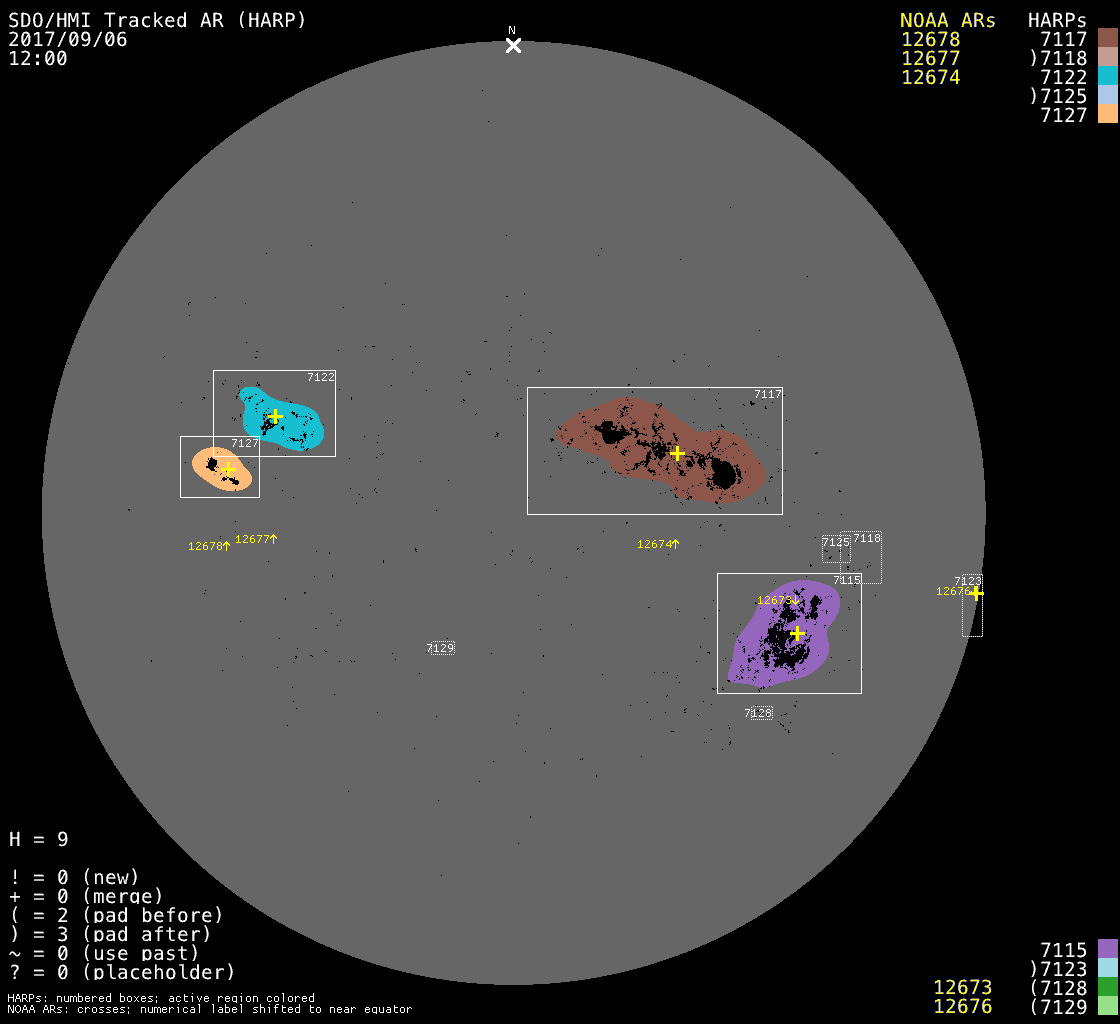
\includegraphics[scale=0.19]{magnetogram_20170906.png}
        \caption{HARPs on 9/6/17.}
        \label{fig:magnetogram_20170906}
    \end{figure}
\end{frame}

\begin{frame}{SHARP Parameter Data}
    \begin{figure}
        \centering
        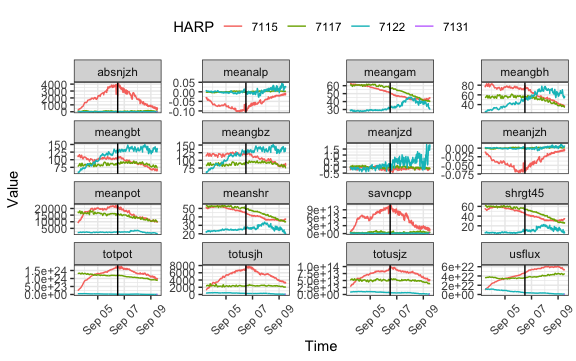
\includegraphics[scale=0.55]{sharp_params_20170906.png}
        \caption{SHARP parameters, 9/3/17-9/9/17}
        \label{fig:sharp_params_20170906}
    \end{figure}
\end{frame}

\begin{frame}{Preprocessing}
    \begin{itemize}
        \item Different ways to put the SHARP parameters on the same scale:
        \begin{itemize}
            \item Standardization
            \item Rank-transforming
            \item Pareto-transforming
        \end{itemize}
        \item Covariates are lagged:
        \begin{figure}
            \centering
            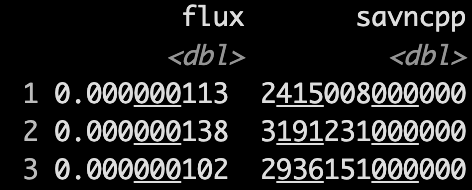
\includegraphics[scale=0.4]{unlagged_vars.png}
            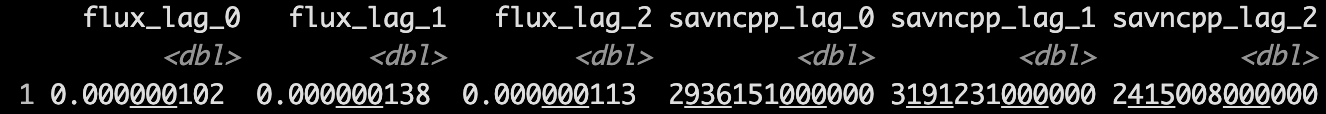
\includegraphics[scale=0.4]{lagged_vars.png}
        \end{figure}
        \item Dimensionality reduction
        \begin{itemize}
            \item PCA
            \item Spline-based dimensionality reduction 
        \end{itemize}
    \end{itemize}
\end{frame}

\begin{frame}{Preprocessing}
    \begin{figure}
        \centering
        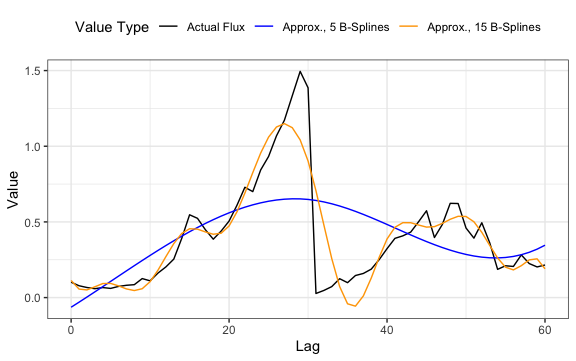
\includegraphics[scale=0.5]{spline_plots.png}
        \caption{A sequence of flux values and its B-spline basis approximations.}
        \label{fig:spline_plots}
    \end{figure}
\end{frame}

\begin{frame}{Optimal Prediction}
    \begin{itemize}
    \item General problem: given a response $Y$ and covariates $X$, predict whether $Y > F_Y^{-1}(p)$ using $X$.
    \item Idea: predict that $Y > F_Y^{-1}(p)$ when $g(X) \in B$ for some $g$, $B$.
    \item $g(X)$ should be calibrated, i.e.,
    \[
    \P(g(X) \in B) = \P(Y > F_Y^{-1}(p)) = 1 - p.
    \]
    \item Set $B = [F_{g(X)}^{-1}(p), \infty)$, i.e., predict that $Y > F_Y^{-1}(p)$ when $g(X) > F_{g(X)}^{-1}(p)$.
    \item \textbf{What should $g$ be?}
    \end{itemize}
\end{frame}

\begin{frame}{Optimal Prediction}
    \begin{theorem} The optimal predictor of $1_{\{Y > F_Y^{-1}(p)\}}$ in terms of $X$ is of the form $1_{\{h(X) > F_{h(X)}^{-1}(p)\}}$, where
    \[
    h(x) = \frac{f_1(x)}{f_0(x)} = 
    \frac{p \int_{F_Y^{-1}(p)}^{\infty} f_{X, Y}(x, y)\,dy}{(1 - p)\int_{-\infty}^{F_Y^{-1}(p)} f_{X, Y}(x, y)\,dy}.
    \]
    More precisely, for every other calibrated predictor $1_{\{g(X) > F_{g(X)}^{-1}(p)\}}$, we have
    \begin{align*}
    \P[Y > F_Y^{-1}(p) \mid g(X) > F_{g(X)}^{-1}(p)] \le \P[Y > F_Y^{-1}(p) \mid h(X) > F_{h(X)}^{-1}(p)]
    \end{align*}
    \end{theorem}
\end{frame}

\begin{frame}{Optimal Prediction}
    \begin{corollary} Consider the additive error model
    \[
    Y = m(X) + \sigma(X)\epsilon,
    \]
    where $X \ind \epsilon$ and $\sigma(X) > 0$.
    The optimal predictor is 
    \[
    h(x) = \frac{m(x) - F_Y^{-1}(p)}{\sigma(x)}.
    \]
    \end{corollary}
\end{frame}

\section{Prediction Methodologies}

\begin{frame}{Tail Dependence Approach}
    The \textbf{tail dependence coefficient} between random variables $U$ and $V$ is defined as
    \[
    \lambda(U, V) = \lim_{p \to 1^{-}} \P[V > F_V^{-1}(p) \mid U > F_U^{-1}(p)].
    \]
    Note that
    \begin{align*}
        \lambda(U, V) &= \lim_{p \to 1^{-}} \frac{\P[U > F_U^{-1}(p), V > F_V^{-1}(p)]}{\P[U > F_U^{-1}(p)]} \\
        &= \lim_{p \to 1^{-}} \frac{\P[U > F_U^{-1}(p), V > F_V^{-1}(p)]}{1 - p} \\ 
    \end{align*}
\end{frame}

\begin{frame}{Tail Dependence Approach}
    Idea: find $g$ so that $g(X)$ and $Y$ have high tail dependence, predict using $g(X)$.

    \medskip
    
    One estimator of the tail dependence coefficient:
    \[
    \hat{\lambda}_p(Y, g(X)) = \frac{1}{n(1 - p)}\sum_{i = 1}^n I(g(X_i) \ge \hat{F}_{g(X)}^{-1}(p))I(Y_i \ge \hat{F}_{Y}^{-1}(p));
    \]
    $p$ is fixed, and $\hat{F}_{g(X)}^{-1}(p)$ and $\hat{F}_{Y}^{-1}(p)$ estimate the $p$th quantiles of $g(X)$ and $Y$, respectively.
\end{frame}

\begin{frame}{Tail Dependence Approach}
    Given data $(X_1, Y_1), \ldots, (X_n, Y_n)$ and some class $\mathcal{C}$ of functions, compute $g$ as 
    \[
    \argmax_{\tilde{g} \in \mathcal{C}} [\hat{\lambda}_p(Y, \tilde{g}(X)) + \text{penalty}].
    \]
    Some choices for $\mathcal{C}$:
    \begin{itemize}
        \item $\mathcal{C}_{\text{LM}} = \{\tilde{g} : \tilde{g}(x) = x^{\top}\beta, \beta \in \mathbb{R}^d\}$
        \item $\mathcal{C}_{\text{GAM}} = \left\{\tilde{g} : \tilde{g}(x) = \sum_{i = 1}^d s_i(x_i)\right\},$
        where the $s_i$'s are $k$-knot natural cubic splines.
    \end{itemize}
    If $\mathcal{C}$ is $\mathcal{C}_{\text{LM}}$ or $\mathcal{C}_{\text{GAM}}$, then
    \[
    \text{penalty} = \eta\|\beta - \hat{\beta}_{\text{prev}}\|_2.
    \]
\end{frame}

\begin{frame}{Tail Dependence Approach}
    Prediction works as follows. With the data $(X_1, Y_1), \ldots, (X_n, Y_n)$,
    \begin{itemize}
        \item set $\hat{F}_{g(X)}^{-1}(p)$ to the $p$th sample quantile of $\{g(X_1), \ldots, g(X_n)\}$
        \item given a new observation $X_*$, predict that $Y_* > F_{Y}^{-1}(p)$ if $g(X_*) > \hat{F}_{g(X)}^{-1}(p)$
    \end{itemize}
\end{frame}

\begin{frame}{TSS}
    The True Skill Statistic, used to measure performance, is
    \[
    TSS = \frac{TP}{TP + FN} - \frac{FP}{FP + TN}
    \]
\end{frame}

\begin{frame}{Tail Dependence Approach}
    \begin{figure}
        \centering
        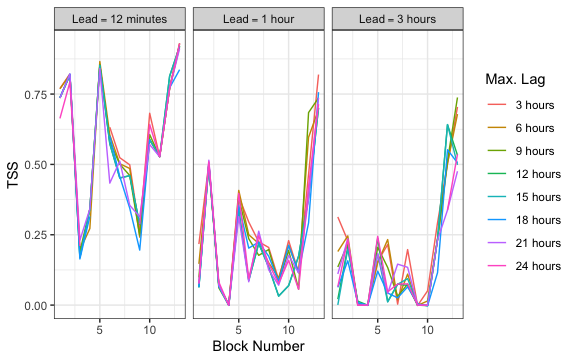
\includegraphics[scale=0.5]{group02_cv_study01_tss.png}
        \caption{Cross-validation results, $\mathcal{C}_{\text{LM}}$.}
        \label{fig:group05_cv_study01_tss}
    \end{figure}
\end{frame}

\begin{frame}{Tail Dependence Approach}
    \begin{figure}
        \centering
        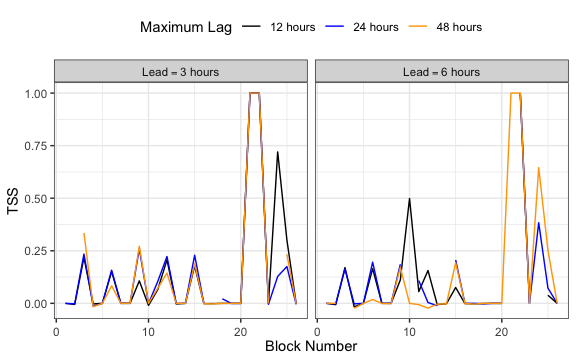
\includegraphics[scale=0.5]{group05_cv_study01_tss.png}
        \caption{Cross-validation results, $\mathcal{C}_{\text{LM}}$, 15 B-splines.}
        \label{fig:group05_cv_study01_tss}
    \end{figure}
\end{frame}

\begin{frame}{Future Work}
    \begin{itemize}
        \item Tail dependence approach: consider functions $g(X)$ that are copulas or neural networks
        \item Logistic regression
        \item State space models
    \end{itemize}
\end{frame}

\begin{frame}{References}
    \nocite{*}
    \printbibliography
\end{frame}

\end{document}